\documentclass[12pt]{article}
\usepackage{setspace}
\usepackage{geometry}
\usepackage{hyperref}
% \usepackage{mathptmx} % times new roman
\usepackage{tocloft} % table of contents
\usepackage{graphicx}
\usepackage[
    backend=bibtex,
    style=ieee,
]{biblatex}
\addbibresource{refs.bib}
% ========================================== %
% document options
\doublespacing
\raggedright
\geometry{ 
    a4paper,
    margin=1in,
    lmargin=1.5in
}

\usepackage{xcolor}
\hypersetup{
    colorlinks,
    linkcolor={red!50!black},
    citecolor={blue!50!black},
    urlcolor={blue!80!black}
}
% ========================================== %
% section notations
\renewcommand{\thesection}{}
\renewcommand{\thesubsection}{}
\renewcommand*\contentsname{ 
    {\MakeUppercase{Table of Contents}} 
}
\renewcommand*\listfigurename{ 
    {\section{{LIST OF FIGURES}}} 
}
\renewcommand*\listtablename{
    {\section{{LIST OF TABLES}}} 
}
% ========================================== %
% custom variables
\newcommand{\thesistitle}{
    {\Large A comparative analysis of texture analysis methods on
ant images}
}
\newcommand{\toppage}{\vspace*{0.3in}}
% ========================================== %

\begin{document}
\pagenumbering{roman}
% ========================================== %
% thesis premable page
\toppage
\begin{center}
    \textbf{\MakeUppercase{\thesistitle}}
    \vspace{1in}

    A Thesis Presented to

    The Faculty of the Computer Science Department
    \vspace{1in}

    by
    \vspace{0.5in}

    Noah Gardner
    \vspace{1in}

    In Partial Fulfillment

    of Requirements for the Degree

    Master of Science in Computer Science

    \vspace{1in}
    Kennesaw State University

    May 2022
\end{center}
\thispagestyle{empty}
\newpage

% ========================================== %
% agreement
\toppage
\noindent In presenting this thesis as a partial fulfillment of the requirements
for an advanced degree from Kennesaw State University, I agree that the
university library shall make it available for inspection and circulation in
accordance with its regulations governing materials of this type. I agree that
permission to copy from, or to publish, this thesis may be granted by the
professor under whose direction it was written, or, in his absence, by the dean
of the appropriate school when such copying or publication is solely for
scholarly purposes and does not involve potential financial gain. It is
understood that any copying from or publication of, this thesis which involves
potential financial gain will not be allowed without written permission.
\vspace{2in}

\def\dotsign{\xleaders\hbox to .2em{\d{}}\hfill\d{}}
\begin{center}
    \makebox[.5\linewidth][r]\dotsign\smallskip\\
    Noah Gardner
\end{center}
\newpage

% ========================================== %
% notice to borrowers
\toppage
\begin{center}
    \textbf{\underline{Notice to Borrowers}}
\end{center}
\vspace{0.5in}

\noindent Unpublished theses deposited in the Library of Kennesaw State
University must be used only in accordance with the stipulations prescribed by
the author in the preceding statement.
\vspace{0.5in}

\noindent The author of this thesis is:
\begin{center}
    Noah Gardner

    1100 S Marietta Parkway

    Marietta, GA 30060
\end{center}

\noindent The director of this thesis is:
\begin{center}
    Chih-Cheng Hung

    1100 S Marietta Parkway

    Marietta, GA 30060
\end{center}
\vspace{0.5in}

\noindent Users of this thesis not regularly enrolled as students at Kennesaw
State University are required to attest acceptance of the preceding stipulations
by signing below. Libraries borrowing this thesis for the use of their patrons
are required to see that each user records here the information requested.
\vspace{0.3in}

\noindent
Name of user \hspace{0.2in} Address \hspace{0.2in} Date \hspace{0.2in} Type of
use (examination only or copying)
\newpage

% ========================================== %
% abstract preamble page title page
\toppage
\begin{center}
    \textbf{\MakeUppercase{\thesistitle}}
    \vspace{1in}

    An Abstract of

    A Thesis Presented to

    The Faculty of the Computer Science Department
    \vspace{1in}

    by
    \vspace{0.5in}

    Noah Gardner
    \vspace{1in}

    In Partial Fulfillment

    of Requirements for the Degree

    Master of Science in Computer Science

    \vspace{1in}
    Kennesaw State University

    May 2022
\end{center}
\newpage

% ========================================== %
% abstract page
\toppage
\begin{center}
    \section{ABSTRACT}
\end{center}
\vspace{0.5in}

\noindent There is a large variety of ant species, and most species are diverse
in terms of size, shape, behaviors, and especially skin (cuticle) textures.
However, the significance of ant cuticle texture is not widely researched. This
research employs modern machine learning methods such as texture analysis and
classification with CNN and clustering to automatically group similar ant
species to allow for the study of influences cuticle texture on ant ecology.
\newpage

% ========================================== %
% advisor preamble
\toppage
\begin{center}
    \textbf{\MakeUppercase{\thesistitle}}
    \vspace{1in}

    A Thesis Presented to

    The Faculty of the Computer Science Department
    \vspace{1in}

    by
    \vspace{0.5in}

    Noah Gardner
    \vspace{1in}

    In Partial Fulfillment

    of Requirements for the Degree

    Master of Science in Computer Science
    \vspace{0.5in}

    Advisor: Dr. Chih-Cheng Hung
    \vspace{0.5in}

    Kennesaw State University

    May 2022
\end{center}
\newpage

% ========================================== %
% quote page
\toppage
Never fail to have this attitude of mind, go forward without hurry, learn the
essence of things through frequent experiences, taking advantage of every
occasion. Fight against all kinds of people and be aware of their mind. Follow a
road that is a thousand leagues long one step at a time. Be without haste and be
convinced that all these practices are the duty of a bushi. Be victorious today
over what you were yesterday; tomorrow be victorious over your clumsiness and
then also over your skill. Practice in accordance with what I have written
without letting your mind deviate from the way.

\vspace{0.5in}
\hspace*{\fill} Miyamoto Musashi \footnote{Miyamoto Musashi, The Book of Five
    Rings}
\newpage

% ========================================== %
% acknowledgements page
\toppage
\begin{center}
    \section{ACKNOWLEDGEMENTS}
\end{center}
\vspace{0.5in}

\noindent It is a bit cliche for an author to thank their family. Nevertheless,
I would have given up a long time ago without the support of my family. So, I
would like to thank my loving family for their support throughout the completion
of my graduate degree. I would also like to thank Dr. Chih-Cheng Hung for his
mentorship for my thesis and for his guidance in my other research projects.
Next, I would like to thank Dr. Zhiling Long for his insights for machine
learning and texture analysis. Finally, I would like to thank Dr. Coskun Tekes
for providing the Lambda Labs GPU server for my experiments.
\newpage

% ========================================== %
% table of contents
\begin{center}
    \tableofcontents
\end{center}
\newpage

% ========================================== %
% list of figures
\begin{center}
    \listoffigures
\end{center}
\newpage

% ========================================== %
% list of tables 
\begin{center}
    \listoftables
\end{center}
\newpage

% ========================================== %
% begin content
\pagenumbering{arabic}
\setlength{\parskip}{\baselineskip}

% ========================================== %
% chapter 1 - introduction and background
\section{CHAPTER 1: INTRODUCTION AND BACKGROUND}
\subsection{Introduction}

Insects comprise over half of the world's animal biodiversity
\cite{tihelka_evolution_2021}. Insects are vital to many ecosystem functions,
including nutrient recycling, plant propagation, and maintenance of plant and
animal communities \cite{gullan_insects_2009, berenbaum_bugs_1996}. As technology
advances, systems which can automatically analyze insect-based information are
growing in demand by biologists. Due to the extensive number of insect species,
manual exploration of insect-based information is difficult and often requires
specialized expertise. Therefore, automated entomology is gaining attraction by
both biologists and computer scientists and is expected to be a major
contribution to the future of insect-based research
\cite{martineau_survey_2017}. One of the most commonly used data types for
insect analysis is image data. To develop an image-based system for insect
analysis, we can take advantage of existing work in general image processing and
texture analysis methods.

Texture is an important feature in many applications, such as image processing,
pattern recognition, and computer vision. Analysis of textures can be broken
into three main categories: texture classification, texture segmentation, and
texture synthesis \cite{reed_review_1993}. The process of classifying a texture
into a set of categories and relies on three different approaches. In this
paper, we focus on a \textit{model-based approach} which attempts to extract
parameters to reveal common patterns and use those parameters to automatically
distinguish between different textures \cite{maillard_texture_2003}.

In this work, we explore automated entomology specifically for ants. Although
there is some work regarding grouping ants into categories of similar cuticle,
automated categorization has yet to become an active area of research. In
general, the goal of automated insect classification methods is species
indentification - \textit{i.e.} the identification of species from a set of
observations. Due to the large number of different ant species, large scale ant
species indentification with standard classification methods is not feasible.
Therefore, we must simplify the problem by either other classifying a certain
subset of ant species or by applying categories to the entire set of ant
species.

In many texture analysis methods, the general goal is to automatically
categorize an object into a set of objects with similar texture-based features.
The approach of texture analysis to categorize similarly texture-based objects
corresponds well to the demands of ant identification. Texture analysis has
shown promising results in related fields, such as plant identification
\cite{boudra_plant_2018}. With modern texture analysis methods, the
categorization of ants can be automated and the results can be used to study the
influence of cuticle texture on ant ecology.

\subsection{Research Question}

The overarching question that we wish to address by beginning this research is:
\textit{how does the texture of ant cuticle affect the ant ecology}? However, to
even begin contemplating this question requires a substantial amount of
preliminiary research. One point that is necessary to begin this research is to
propose a method of group ants by texture. Additionally, due to the sheer number
of ant species, an automated effort is necessary to group similar ant species.
Therefore, we start our endeavor with a more straightforward research question:
\textit{are texture analysis methods able to group similar ant species}? By the
end of this research, we will answer this question by demonstrating a variety of
texture analysis methods and comparing their results on a custom dataset.

\subsection{Proposed Approach}

In order to group similar ant species, we require mostly uniform images that
depict the texture of the ant cuticle. We source our raw images from AntWeb
\cite{perrichot_antweb_2012}, a database of ant head images. An example image is
shown in Figure \ref{fig:CASENT0217419}. In general, the ant head images are centered in
the image, facing the front, and share a similar posture. However, some images
may not be centered, show the ant head in a different orientation, or may have a
drastically different resolution from the average image. With some data
preprocessing methods, these ant head images are suitable for traditional
methods of image classification.

\begin{figure}[ht]
    \centering
    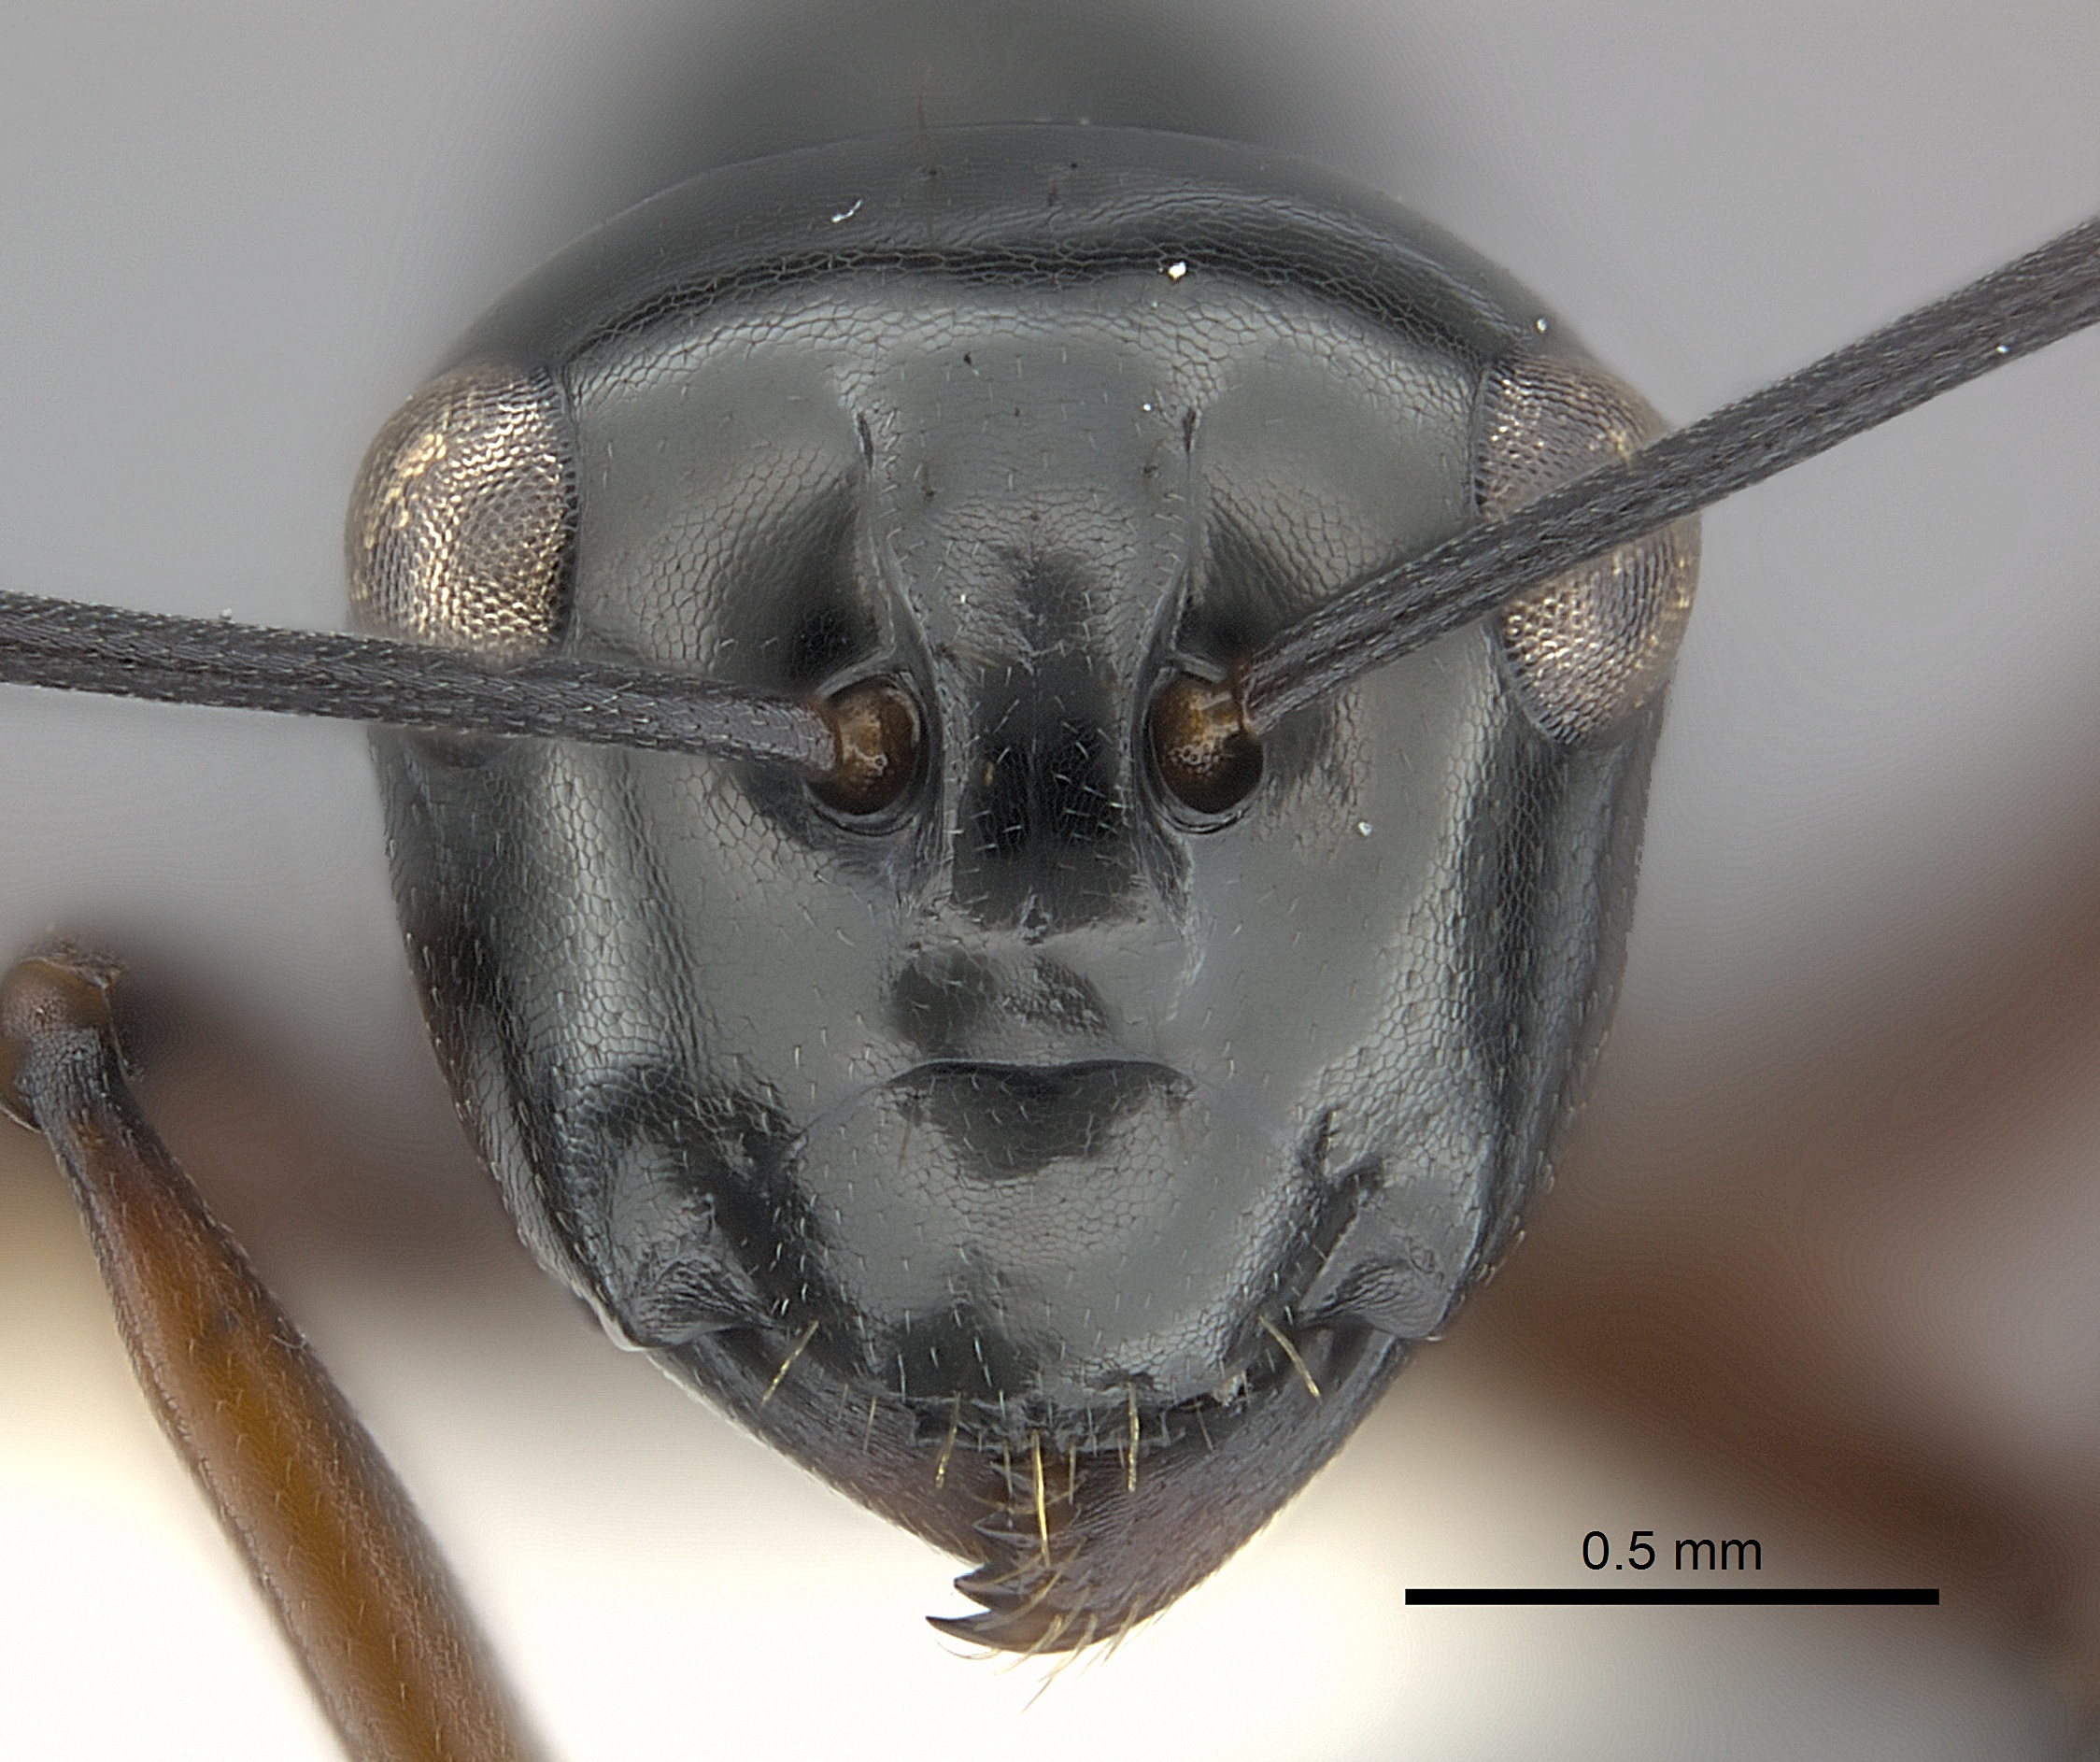
\includegraphics[width=0.8\textwidth]{assets/images/CASENT0217419.jpg}
    \caption{ An example ant head image from AntWeb of species
        \textit{Polyrhachis abbreviata} - specimen
        \href{https://www.antweb.org/bigPicture.do?name=casent0217419&shot=h&number=1}{CASENT0217419}
        by \href{https://www.antweb.org/artist.do?id=92}{Estella Ortega}, from
        \href{https://www.antweb.org}{AntWeb}, is licensed under
        \href{https://creativecommons.org/licenses/by/4.0/}{CC BY 4.0}.}
    \label{fig:CASENT0217419}
\end{figure}

\subsection{Research Impact}

The primary contribution of this research is the development of a unique dataset
for ant cuticle texture classification. Additionally, we compare the results of
state-of-the-art deep learning and texture analysis methods on our proposed
dataset. The secondary contribution is the analysis of the results of these
methods and data analysis.
\newpage
% ========================================== %
% chapter 2 - literature review
\section{CHAPTER 2: LITERATURE REVIEW}

\subsection{Insect Classification}

In this section, we provide an overview of some insect classification methods.

\citeauthor*{lim_performance_2017} apply a CNN-based algorithm for insect
classification \cite{lim_performance_2017}. \citeauthor*{lim_performance_2017}
classify a subset of insect species and families based on the classes available
in the ImageNet dataset \cite{deng_imagenet_2009}. ImageNet is a widely used
dataset of images labeled by experts with millions of images and thousands of
categories \cite{deng_imagenet_2009}. In the ImageNet dataset, there are some
categories that specify the class of the insect on a species level,
\textit{e.g.} \textit{monarch butterfly} and \textit{ringlet butterfly} as well
as some categories that specify the class of the insect on a family level,
\textit{e.g.} \textit{ant}, \textit{fly}, and \textit{bee}
\cite{imagenet_labels}. \citeauthor*{lim_performance_2017} use a modified
AlexNet architecture and experiment on how different numbers of kernels affect
the performance of the model \cite{lim_performance_2017}.
\citeauthor*{glick_insect_2016} employ a similar approach by classifying 277
insect classes from ImageNet using a hierarchical CNN \cite{glick_insect_2016}.
The results from \citeauthor*{lim_performance_2017} and
\citeauthor*{glick_insect_2016} suggest that a CNN is capable of differentiating
between different hierarchical classes of insects. In our research, we are
interested in the classification of ant images of a hierarchical level
in-between species and family.

% bees

% fruit flies

\newpage
% ========================================== %
% chapter 3 - methodology
\section{CHAPTER 3: METHODOLOGY}
\newpage
% ========================================== %
% chapter 4 - experimental results and analysis
\section{CHAPTER 4: EXPERIMENTAL RESULTS AND ANALYSIS}

\subsection{Environment}
\newpage
% ========================================== %
% chapter 5 - conclusion
\section{CHAPTER 5: CONCLUSION}
\newpage

\printbibliography
\end{document}